%%%%%%%%%%%%%%%%%%%%%%%%%%%%%%%%%%%%%%%%%%%%%%%%%%%%%%%%%%%%%%%%%%%%%%%%%%%%%%
  \headerbox{Petri Net in a nutshell}{name=future,column=0,below=problem}{
%%%%%%%%%%%%%%%%%%%%%%%%%%%%%%%%%%%%%%%%%%%%%%%%%%%%%%%%%%%%%%%%%%%%%%%%%%%%%%
   \vspace{1.8mm}
   \noindent{\centering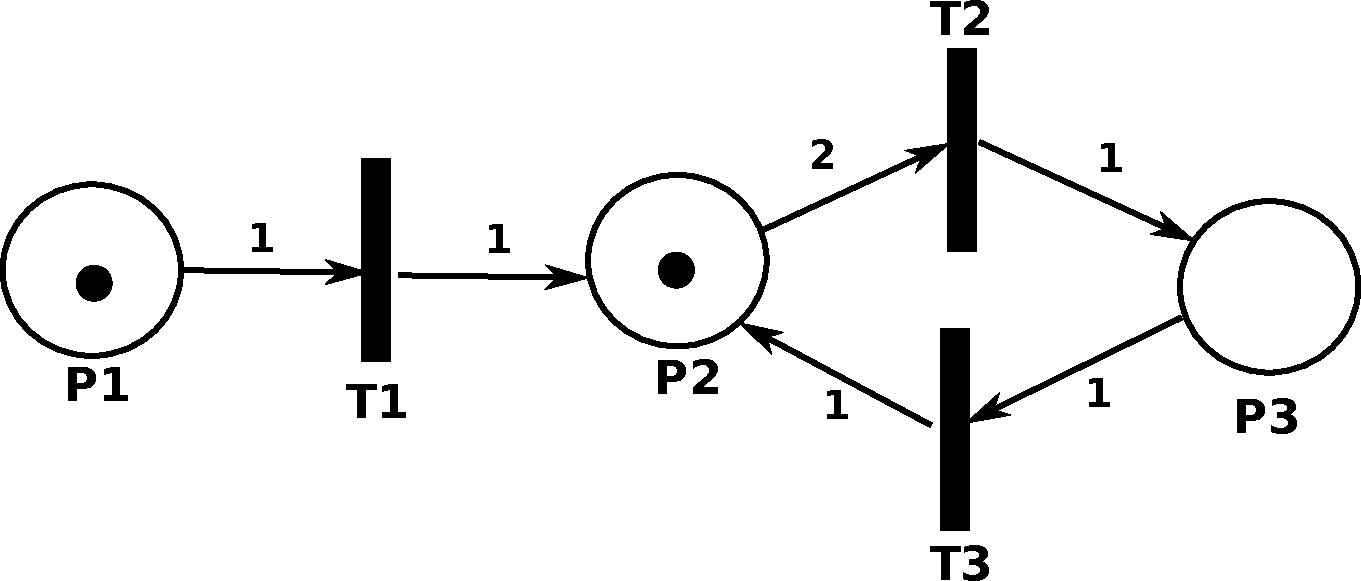
\includegraphics[scale=0.3]{images/petri.pdf}\\}
   \vspace{1.8mm}
A Petri net is a bipartite graph with two types of nodes: 
\begin{itemize}
   \item {\bf \emph{Place (in circle):}} it can contain a 
number of \emph{tokens}, which are drawn as dots and typically represent resources.
   \item {\bf \emph{Marking:}} a mapping from each place $p$ to the number of tokens at $p$.
   \item {\bf \emph{Transition (in solid bar):}} corresponds to events that change the marking.
\end{itemize}
   \vspace{0.4em}
  }

